% Copyright (c) 2017 Alexander Bluhm <bluhm@openbsd.org>
%
% Permission to use, copy, modify, and distribute this software for any
% purpose with or without fee is hereby granted, provided that the above
% copyright notice and this permission notice appear in all copies.
%
% THE SOFTWARE IS PROVIDED "AS IS" AND THE AUTHOR DISCLAIMS ALL WARRANTIES
% WITH REGARD TO THIS SOFTWARE INCLUDING ALL IMPLIED WARRANTIES OF
% MERCHANTABILITY AND FITNESS. IN NO EVENT SHALL THE AUTHOR BE LIABLE FOR
% ANY SPECIAL, DIRECT, INDIRECT, OR CONSEQUENTIAL DAMAGES OR ANY DAMAGES
% WHATSOEVER RESULTING FROM LOSS OF USE, DATA OR PROFITS, WHETHER IN AN
% ACTION OF CONTRACT, NEGLIGENCE OR OTHER TORTIOUS ACTION, ARISING OUT OF
% OR IN CONNECTION WITH THE USE OR PERFORMANCE OF THIS SOFTWARE.

\documentclass[14pt]{beamer}
\usetheme{Frankfurt}
\usepackage{tikz}
\usepackage{bold-extra}
\author{Alexander Bluhm}
\title{Never Loose a Syslog Message}
\institute{\url{bluhm@openbsd.org}}
\date{\today}

\begin{document}

\begin{frame}
\titlepage
\end{frame}

\begin{frame}{Agenda}
\tableofcontents
\end{frame}

\section{Motivation}

\begin{frame}{Why reliable logging?}
\begin{itemize}
    \item system analysis
    \item attacker tries to prevent log
    \item required by common criteria
\end{itemize}
\end{frame}

\begin{frame}{What can go wrong?}
\begin{itemize}
    \item UDP for remote logs
    \item UNIX datagram for local logs
    \item file descriptors
    \item chroot environment
    \item timestamps and time zones
\end{itemize}
\end{frame}

\section{Starting Position}

\begin{frame}{Message Flow}
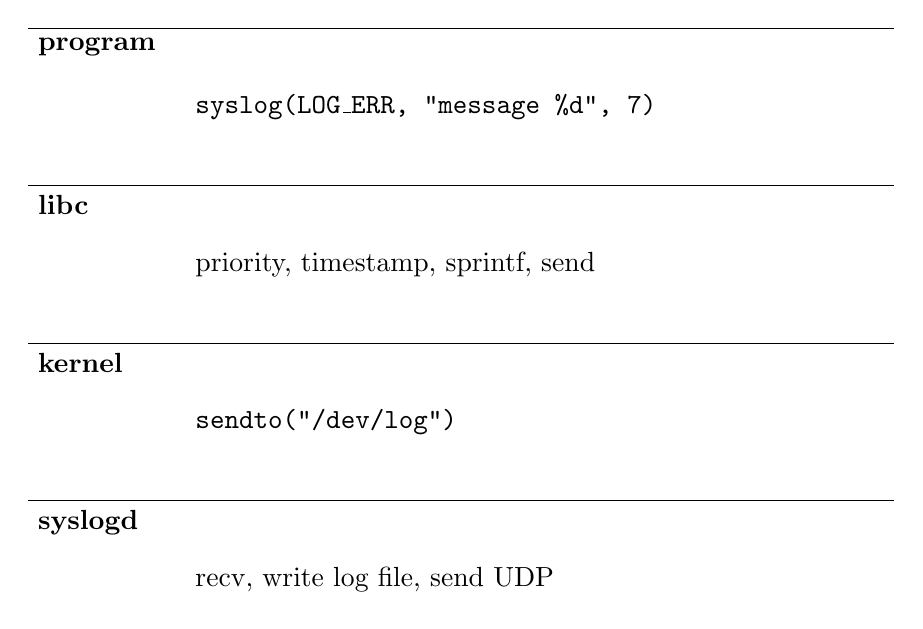
\begin{tikzpicture}
\draw
    ++(0,-2) node[anchor=north west]{\textbf{program}} -- +(11,0)
    +(2,-1) node[anchor=west]{\texttt{syslog(LOG\_ERR, "message \%d", 7)}}
    ++(0,-2) node[anchor=north west]{\textbf{libc}} -- +(11,0)
    +(2,-1) node[anchor=west]{priority, timestamp, sprintf, send}
    ++(0,-2) node[anchor=north west]{\textbf{kernel}} -- +(11,0)
    +(2,-1) node[anchor=west]{\texttt{sendto("/dev/log")}}
    ++(0,-2) node[anchor=north west]{\textbf{syslogd}} -- +(11,0)
    +(2,-1) node[anchor=west]{recv, write log file, send UDP};
\end{tikzpicture}
\end{frame}

\begin{frame}{Priority, Facility, Level, Severity, Options}
    \texttt{openlog("ftpd", LOG\_PID|LOG\_CONS, LOG\_FTP)}\\
    \texttt{syslog(LOG\_INFO, "\%s logged in", user)}

    \vspace{.5cm}
    \texttt{\#define LOG\_FTP  (11<<3) /* ftp daemon */}\\
    \texttt{\#define LOG\_INFO 6       /* informational */ }

    \vspace{.5cm}
    \texttt{<94>Sep 24 09:45:00 localhost ftpd[4711]:\ bluhm logged in}
\end{frame}

\section{Improvements}

\begin{frame}{/dev/log}
Problems with \texttt{/dev/log} UNIX socket
\begin{itemize}
    \item needs file descriptor
    \item use \texttt{LOG\_NDELAY}
    \item reconnect after \texttt{SIGHUP} syslogd
    \item needs UNIX socket in chroot
    \item needs \texttt{pledge("unix")}
    \item LOG\_CONS is even worse
\end{itemize}
\end{frame}

\begin{frame}{sendsyslog}
    New system call sendsyslog(2)

    \vspace{.5cm}
    \texttt{int \\
    sendsyslog(const void *msg, size\_t len, int flags)}

    \vspace{.5cm}
    \texttt{sendsyslog("<94>Sep 24 09:45:00 localhost ftpd[4711]:\ 
	bluhm logged in", 57, LOG\_CONS)}
\end{frame}

\begin{frame}{using sendsyslog}
    Syslogd does
\begin{itemize}
    \item create socketpair
    \item register one end with \texttt{ioctl(LIOCSFD)}
    \item receive form other end
\end{itemize}
    \vspace{.5cm}
    Kernel does
\begin{itemize}
    \item send to syslogd's socketpair
    \item write to console if necessary
    \item count errors
\end{itemize}
\end{frame}

\begin{frame}{Error Handling}
    \texttt{\textbf{void}} \\
    \texttt{syslog(int prio, const char *msg, ...)}
\begin{itemize}
    \item libc cannot return error
    \item program cannot log error
\end{itemize}
    Kernel sendsyslog can do it
\begin{itemize}
    \item count failed send to syslogd
    \item write message to syslog when it works again
\end{itemize}
    \texttt{sendsyslog:\ dropped 2 messages, error 57}
\end{frame}

\begin{frame}{Timestamp}
\end{frame}

\begin{frame}{Logging without Libc}
\end{frame}

\begin{frame}{dmesg}
\end{frame}

\begin{frame}{Certificates}
\end{frame}

\begin{frame}{Tests}
\end{frame}

\begin{frame}{TODO}
\begin{itemize}
    \item File system full recovery
    \item Memory buffer overflow
\end{itemize}
\end{frame}

\end{document}
